\chapter{Multimodal Fusion for Species Classification in Camera Trap Workflows}\label{cap:experiment_02}

\section{Introduction}

Camera trap monitoring is an important tool for biodiversity assessment, but the large volume of images produced by these systems makes manual annotation costly and time-consuming. Automated species classification can support ecological workflows by reducing the effort required to inspect and label collected images. This chapter addresses species classification in camera trap images under a zero-shot setting, that is, without task-specific training or fine-tuning on the target datasets.

The method under study, referred to as \textit{WildMatch-CLIP-LLM-Fusion}, integrates complementary visual and textual signals in a multimodal inference pipeline. The first signal is obtained directly from the image by means of CLIP, which measures similarity between the input image and textual species descriptions represented in a shared vision-language embedding space. The second signal is derived from natural-language descriptions of the image generated by a vision-capable large language model, which are subsequently compared against species descriptions encoded with ModernBERT. These two score vectors are then combined through a weighted linear fusion strategy to produce the final species ranking.

A central characteristic of the proposed approach is that all components operate with pre-trained weights and no gradient-based optimisation is performed for the target task. The pipeline therefore relies on the combination of a pre-built textual knowledge base, image-caption generation, visual-text similarity, and score fusion to support classification. The relevance of this experiment lies in evaluating whether such a training-free multimodal strategy can improve zero-shot camera trap species recognition across different datasets and image settings, including both full-frame and cropped images.

\section{Materials and Methods}


\subsection{Pipeline Overview, Inputs, and Data Resources}

The evaluated system is a zero-shot multimodal pipeline designed for animal species classification in camera trap images. For each input image, the method combines: (i) a visual similarity signal obtained from CLIP, and (ii) a textual similarity signal derived from a language-model-generated image description encoded with ModernBERT and matched against species profiles stored in a knowledge base. The final prediction is produced by a weighted linear combination of the two modalities. Because neither CLIP nor the text encoder is adapted to the target domain, the method does not require labelled training data for the evaluated classification task (see Figure \ref{fig:clip_fusion}).


\begin{figure*}[!ht]
\centering
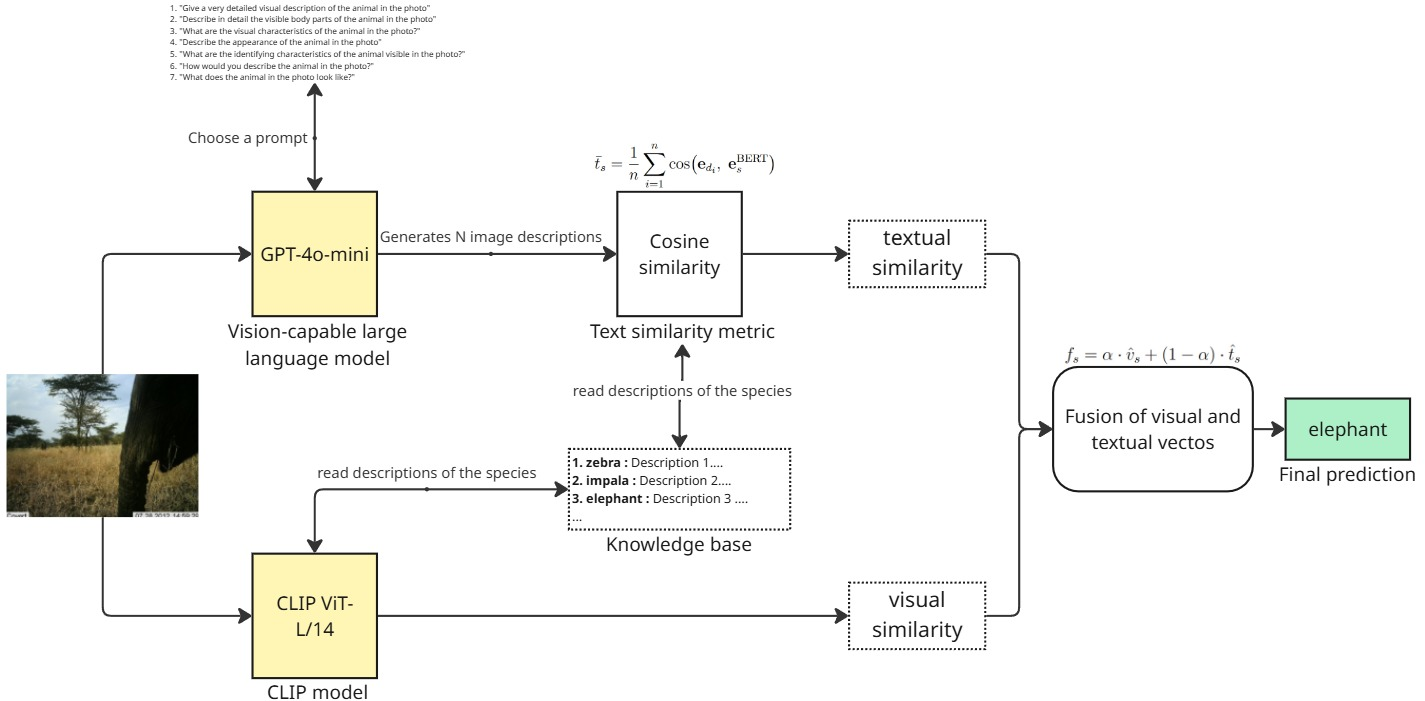
\includegraphics[width=6in]{images/clip_fusion.png}
\caption{WildMatch-CLIP-LLM-Fusion architecture}
\label{fig:clip_fusion}
\end{figure*}

The pipeline takes two inputs for each prediction: a camera trap image and a pre-built knowledge base. Two image variants are considered in the evaluation: full-frame images and cropped images, where the latter correspond to regions containing the animal as obtained through an animal detection step. The knowledge base is represented as a structured JSON resource mapping each candidate species name to a set of textual fields. The key element used during inference is the \textit{Visually Relevant Summary} (VRS), defined as a paragraph-length description of the species' visible appearance. These summaries are generated offline by prompting GPT-4o-mini to extract only photographically observable information from the corresponding Wikipedia article, while excluding non-visual attributes (e.g., measurements, sounds, and smells) and returning a single paragraph.

The experiments are conducted on three camera-trap datasets (Caltech, Serengeti, and WCS). For each dataset, classification is performed over a fixed candidate set corresponding to the species available in that dataset subset. The same candidate set is used to define the class labels and to construct the species entries in the knowledge base used during inference.

\begin{itemize}
\item \textbf{Serengeti (12 species, common names):} zebra, hyenaspotted, warthog, impala, elephant, giraffe, buffalo, guineafowl, ostrich, cheetah, hippopotamus, baboon.
\item \textbf{WCS (10 species, scientific names):} \textit{Equus quagga}, \textit{Bos taurus}, \textit{Loxodonta africana}, \textit{Mitu tuberosum}, \textit{Macaca nemestrina}, \textit{Tapirus terrestris}, \textit{Argusianus argus}, \textit{Psophia leucoptera}, \textit{Panthera onca}, \textit{Hystrix brachyura}.
\item \textbf{Caltech (10 species, common names):} raccoon, coyote, deer, rabbit, bobcat, bird, squirrel, rodent, skunk, lizard.
\end{itemize}

Image preprocessing is minimal and delegated to the CLIP preprocessing transform. The input image is resized, centre-cropped, and normalised according to the model's expected input distribution. No additional augmentation, denoising, or domain-specific preprocessing is applied. The image is loaded and converted to RGB before being passed to the visual encoder.

\subsection{Multimodal Inference Method}

The pipeline consists of three main components: a vision-language model for caption generation, a CLIP-based visual matching branch, and a ModernBERT-based textual matching branch.

A vision-capable large language model, GPT-4o-mini, is used to generate natural-language descriptions of the input image. Rather than relying on a single fixed instruction, the system samples one prompt from a set of paraphrased variants, all aimed at eliciting a detailed visual description of the animal in the photo. This prompt randomisation is intended to encourage descriptive diversity when multiple captions are requested. Each caption is generated with a maximum budget of 500 tokens. In the evaluated configuration, three captions are generated for each image.

The visual branch uses the pre-trained CLIP ViT-L/14 model. CLIP projects both images and texts into a shared 768-dimensional embedding space, allowing similarity computation between the input image and textual species descriptions. Let $\mathbf{e}_{\text{img}}$ denote the $\ell_2$-normalised embedding of the input image. Each species summary from the knowledge base is prepended with a generic camera-trap prompt and encoded through CLIP's text encoder. These text embeddings are computed once and cached for subsequent reuse. For each candidate species $s$, the visual similarity score is defined as the cosine similarity between the image embedding and the cached CLIP text embedding for that species:
\begin{equation}
v_s = \cos\bigl(\mathbf{e}_{\text{img}},\; \mathbf{e}^{\text{CLIP}}_s\bigr).
\end{equation}
This score quantifies the alignment between the visual content of the image and the species-specific textual description represented in the CLIP embedding space.

The textual branch uses \texttt{answerdotai/ModernBERT-base} model. To obtain fixed-length sentence representations, the last hidden state is mean-pooled across all tokens and then $\ell_2$-normalised. Each caption generated by the vision-language model is encoded into a ModernBERT embedding. Similarly, each VRS in the knowledge base is encoded and cached. For each caption $d_i$, cosine similarity is computed against all species embeddings. If $n$ captions are generated, the per-species textual score is obtained by averaging the cosine similarities across captions:
\begin{equation}
\bar{t}_s = \frac{1}{n}\sum_{i=1}^{n}\cos\bigl(\mathbf{e}_{d_i},\; \mathbf{e}^{\text{BERT}}_s\bigr).
\end{equation}
After averaging, the textual score vector is min--max normalised to the interval $[0,1]$.

The final species ranking is obtained by combining the visual and textual score vectors through a weighted linear fusion. When score normalisation is enabled, both the CLIP visual scores and the ModernBERT textual scores are independently min--max normalised to $[0,1]$. The fused score for species $s$ is then computed as:
\begin{equation}
f_s = \alpha \cdot \hat{v}_s + (1-\alpha)\cdot \hat{t}_s,
\end{equation}
where $\hat{v}_s$ and $\hat{t}_s$ are the normalised visual and textual scores, respectively, and $\alpha \in [0,1]$ controls the contribution of each modality. In the evaluated configuration, $\alpha = 0.7$, assigning 70\% of the final score to the CLIP visual branch and 30\% to the textual branch. The predicted label is the species associated with the maximum fused score:
\begin{equation}
\hat{y} = \arg\max_s f_s.
\end{equation}

In addition to the predicted label, the method outputs a confidence value based on the relative margin between the two highest fused scores. Let $f_{(1)}$ and $f_{(2)}$ denote the highest and second-highest fused scores, respectively. The confidence is defined as:
\begin{equation}
c = \frac{f_{(1)}}{f_{(1)} + f_{(2)}}.
\end{equation}
This formulation yields values in the interval $(0.5, 1]$. Scores close to 1 indicate a large separation between the top-ranked and second-ranked candidates, whereas a value near 0.5 corresponds to a near tie.

For each test image, the inference process follows five steps:
\begin{enumerate}
\item The vision-language model generates $n$ captions for the input image.
\item The image is encoded with CLIP, and cosine similarities are computed against the cached CLIP text embeddings of all candidate species.
\item Each generated caption is encoded with ModernBERT, cosine similarities are computed against the cached textual embeddings of all species, and the resulting scores are averaged across captions and normalised.
\item The visual and textual score vectors are independently normalised and fused through the weighted linear combination defined above.
\item The species with the highest fused score is returned as the final prediction together with the confidence estimate.
\end{enumerate}

\subsection{Experimental Protocol and Configuration}

No training, fine-tuning, or parameter optimisation is performed in the evaluated system. CLIP ViT-L/14, ModernBERT-base, and GPT-4o-mini are used with their original pre-trained parameters. The fusion weight $\alpha$ is fixed rather than learned. The construction of the knowledge base is executed as an offline preprocessing step and does not involve gradient-based learning. Accordingly, the complete method operates in a zero-shot regime with respect to the target species classification task.

Evaluation is conducted on the full set of available images for each dataset configuration. No train/test split is performed. The primary metric is top-1 classification accuracy, computed as the proportion of images for which the predicted species matches the ground-truth label. For each image, the system records the true label, predicted label, confidence score, and modality-specific scores for subsequent analysis. The reported experimental results compare the proposed CLIP Fusion approach against a baseline across three datasets---Caltech, Serengeti, and WCS---and under two image settings, namely cropped and full-frame images.

The evaluated configuration uses the following settings:
\begin{itemize}
\item CLIP model: ViT-L/14;
\item text encoder: ModernBERT-base;
\item vision-language model for caption generation: GPT-4o-mini;
\item number of captions per image: $n=3$;
\item fusion weight: $\alpha = 0.7$;
\item score normalisation: min--max scaling to $[0,1]$;
\item CLIP text prompt: a generic camera-trap prefix applied to species summaries;
\item caption generation temperature: 0.7 when $n>1$;
\item maximum caption length: 500 tokens.
\end{itemize}

\section{Experiments and Results}

\subsection{Results Across Datasets and Image Settings}

The experiments evaluate the behaviour of the proposed multimodal pipeline across six principal configurations formed by the combination of three datasets (Caltech, Serengeti, and WCS) and two image types (cropped and full). For each configuration, results are reported for the baseline approach and for the CLIP Fusion pipeline. The main quantities reported are classification accuracy, average confidence, total number of evaluated samples, and number of correct predictions. The comparison between baseline and CLIP Fusion is further summarised in terms of absolute accuracy improvement and change in average confidence.

Table~\ref{tab:exp02_accuracy_summary} summarises the top-1 accuracy results for the six evaluated dataset--image configurations. The proposed CLIP Fusion method outperformed the baseline in four of the six configurations (Caltech cropped, Serengeti cropped, WCS cropped, and WCS full), while slight decreases were observed for Caltech full and Serengeti full.

\begin{table}[t]
\centering
\caption{Top-1 accuracy and number of correct predictions for the baseline and the proposed CLIP Fusion pipeline across datasets and image settings.}
\label{tab:exp02_accuracy_summary}
\resizebox{\textwidth}{!}{%
\begin{tabular}{l l r c c c r r}
\hline
\textbf{Dataset} & \textbf{Image} & \textbf{Samples} & \textbf{Acc. (Base)} & \textbf{Acc. (Fusion)} & \textbf{$\Delta$Acc. (pp)} & \textbf{Correct (Base)} & \textbf{Correct (Fusion)} \\
\hline
Caltech & Cropped & 1000 & 68.3\% & 73.5\% & +5.20 & 683 & 735 \\
Caltech & Full & 1000 & 58.1\% & 58.0\% & $-0.10$ & 581 & 580 \\
Serengeti & Cropped & 1200 & 67.0\% & 68.75\% & +1.75 & 804 & 825 \\
Serengeti & Full & 1200 & 66.42\% & 65.25\% & $-1.17$ & 797 & 783 \\
WCS & Cropped & 1000 & 58.2\% & 60.7\% & +2.50 & 582 & 607 \\
WCS & Full & 1000 & 72.1\% & 76.4\% & +4.30 & 721 & 764 \\
\hline
\end{tabular}%
}
\end{table}

The absolute accuracy improvements of CLIP Fusion relative to the baseline (Table~\ref{tab:exp02_accuracy_summary}) ranged from $-1.17$ to +5.20 percentage points. Across all six configurations, the average reported improvement was 2.08 percentage points. The largest improvement was obtained for Caltech cropped images (+5.20 pp), while the largest decrease relative to baseline occurred for Serengeti full images ($-1.17$ pp). Table~\ref{tab:exp02_accuracy_summary} also reports the sample counts and the absolute numbers of correct predictions. The most pronounced gains in absolute numbers of correctly classified images were obtained for Caltech cropped (from 683 to 735 correct predictions) and WCS full (from 721 to 764).

\subsection{Confidence Analysis}

Average confidence increased for CLIP Fusion in all reported baseline comparisons, regardless of whether accuracy improved (Table~\ref{tab:exp02_confidence_summary}). The corresponding confidence changes ranged from +7.83 to +11.40 percentage points. The largest increase in average confidence was observed for Caltech full images, even though this configuration did not improve in terms of classification accuracy.

\begin{table}[t]
\centering
\caption{Average confidence for the baseline and the proposed CLIP Fusion pipeline across datasets and image settings.}
\label{tab:exp02_confidence_summary}
\begin{tabular}{l l c c}
\hline
\textbf{Dataset} & \textbf{Image} & \textbf{Conf. (Base)} & \textbf{Conf. (Fusion)} \\
\hline
Caltech & Cropped & 86.87\% & 96.50\% \\
Caltech & Full & 84.00\% & 95.40\% \\
Serengeti & Cropped & 88.78\% & 96.69\% \\
Serengeti & Full & 86.50\% & 96.06\% \\
WCS & Cropped & 88.07\% & 96.80\% \\
WCS & Full & 87.83\% & 95.67\% \\
\hline
\end{tabular}
\end{table}

\section{Discussion}

The reported results indicate that the integration of CLIP-based visual matching and language-model-assisted textual matching can improve zero-shot species classification performance in several camera trap scenarios. In particular, the proposed fusion strategy achieved higher top-1 accuracy in four of the six main evaluated configurations, with gains ranging from 1.75 to 5.20 percentage points. The largest positive effects were observed for cropped images in Caltech and for full images in WCS.

At the same time, the results do not indicate uniform improvement across all settings. In full-image configurations for Caltech and Serengeti, the baseline slightly outperformed the proposed fusion approach. This outcome suggests that the contribution of the additional textual branch and the weighted fusion mechanism is dependent on the dataset and image setting under evaluation. Based on the reported experiments alone, the method should therefore be interpreted as beneficial in several, but not all, tested conditions.

The confidence analysis shows a consistent increase in average confidence for CLIP Fusion across all six baseline comparisons. However, these increases in confidence do not always coincide with higher classification accuracy. This is evident in the Caltech full and Serengeti full settings, where CLIP Fusion produced higher average confidence despite lower accuracy than the baseline. Therefore, within the reported experimental evidence, confidence values derived from the fused-score margin appear to reflect score separation between top-ranked classes, but not necessarily improved correctness in every configuration.

The results also illustrate the effect of combining complementary modalities without task-specific training. The visual branch directly compares the input image with species descriptions in CLIP space, while the textual branch introduces an intermediate image description generated by a vision-language model and matched against species summaries with ModernBERT. The observed improvements in four configurations support the view that these two branches can provide complementary information under zero-shot inference. Nevertheless, the reported results do not isolate the independent contribution of each component beyond the comparison to the baseline and the aggregate fusion outcomes.

Some limitations are explicitly identifiable from the described implementation and evaluation protocol. First, the pipeline performs no train/test split and evaluates on all available images. Consequently, the reported results are limited to this evaluation setup and do not include an analysis of generalisation under separate training and testing partitions. Second, the ModernBERT representations are obtained by mean-pooling token embeddings rather than using a dedicated sentence-embedding model, which may be suboptimal for semantic similarity. Third, the method depends on an offline-generated knowledge base whose visually relevant summaries are derived from Wikipedia through GPT-4o-mini prompting. The reported text does not provide an independent evaluation of the effect of summary quality on final classification performance.

A further point concerns the mechanism used for multiple captions. Although the implementation name suggests a voting procedure, the actual method averages textual similarity scores across captions before fusion. This distinction is relevant for interpreting the behaviour of the system, because the reported results correspond to score aggregation rather than label-level majority voting.

Overall, the experiment supports the feasibility of a training-free multimodal classification pipeline for camera trap species recognition. The evidence provided by the reported results shows that this approach can improve top-1 accuracy in several configurations while maintaining a consistent increase in average confidence, although the gains are not universal across all datasets and image types.

\section{Final Remarks}

This chapter described a zero-shot multimodal experiment for species classification in camera trap images based on the \textit{WildMatch-CLIP-LLM-Fusion} pipeline. The method combines a CLIP-derived visual similarity signal with a textual similarity signal obtained from GPT-4o-mini image descriptions and ModernBERT-based semantic matching against species summaries stored in a knowledge base. Final predictions are produced through weighted linear fusion, with no training or fine-tuning performed for the target task.

The reported evaluation showed that the fusion strategy improved top-1 accuracy in four out of six baseline comparisons, with an average gain of 2.08 percentage points across the evaluated configurations. The strongest improvements were observed for Caltech cropped images and WCS full images, while slight performance decreases were observed in two full-image settings. Average confidence increased in all comparisons, although these increases did not always correspond to higher accuracy.

Within the context of this thesis, the experiment contributes a concrete example of how multimodal pre-trained models can be integrated into camera trap workflows without requiring task-specific model training. The results indicate that such integration can be effective under several zero-shot evaluation settings, while also highlighting limitations related to dataset dependence, confidence interpretation, encoder choice, and evaluation protocol.